\section{Procedure}
\subsection{DFT and DFT+U calculation on $\ce{TiO_2}$}
Rutile has a tetragonal unit cell, with two titanium and four oxygen atoms inside. A sketch of a unit cell is given in \cref{fig:rutile}.
\begin{figure}
    \centering
    \begin{subfigure}[t]{0.48\textwidth}
        \centering
        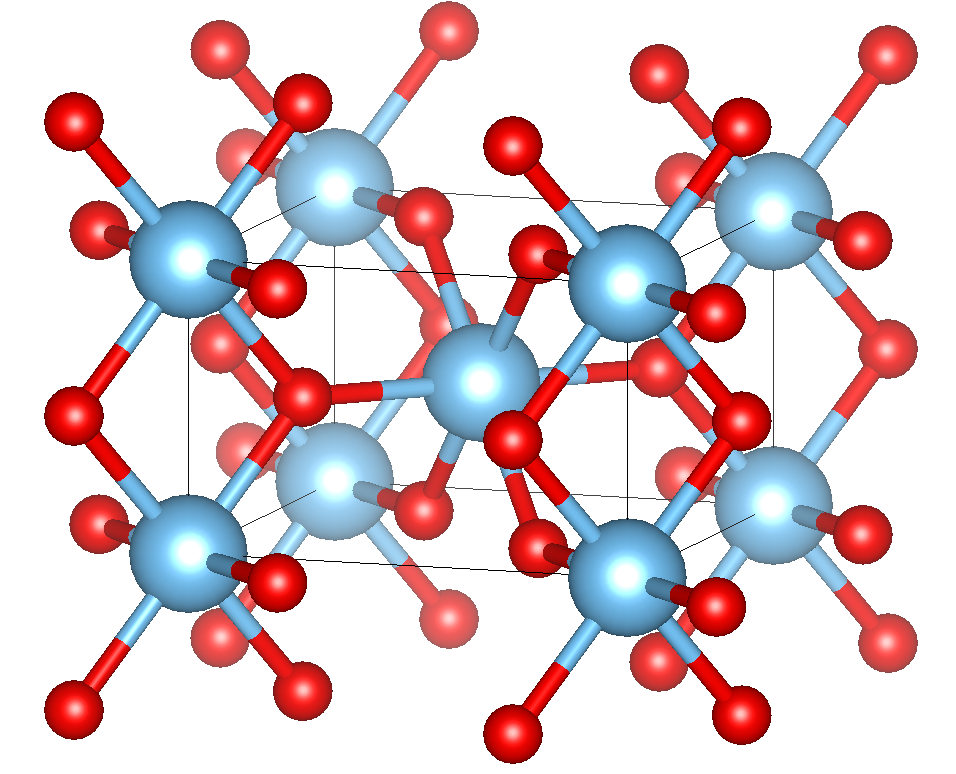
\includegraphics[width=1\textwidth]{figures/rutile.png}
        \caption{Unit cell}
        \label{fig:rutile}
    \end{subfigure}
    \hfill
    \begin{subfigure}[t]{0.48\textwidth}
        \centering
        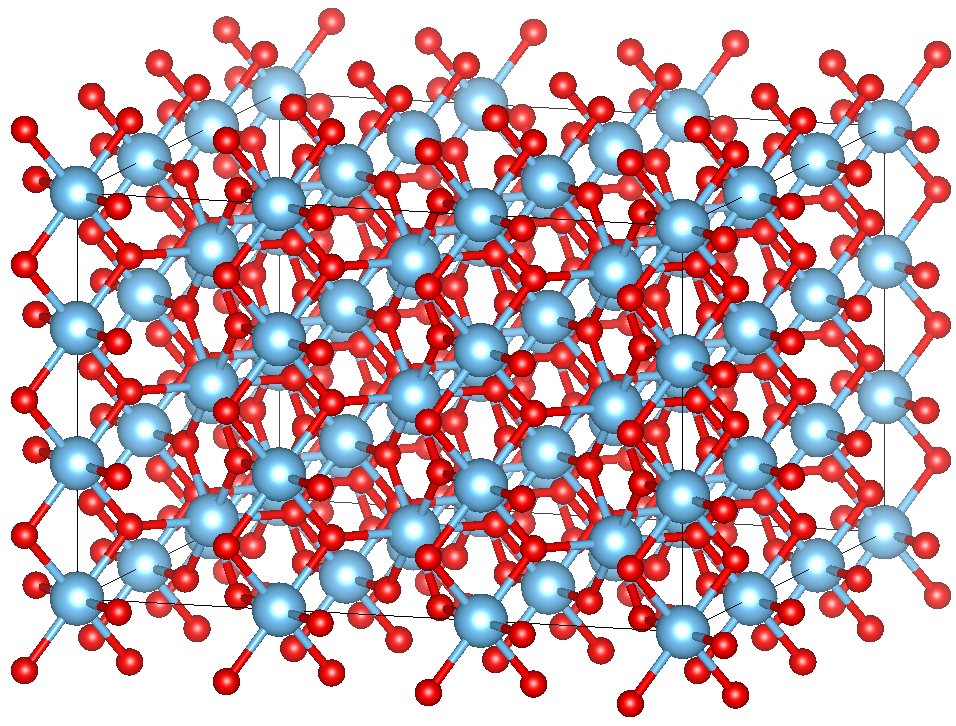
\includegraphics[width=1\textwidth]{figures/supercell.png}
        \caption{$3\times3\times3$ supercell}
        \label{fig:supercell}
    \end{subfigure}
    \caption{Rutile unit cell and supercell. Titanium is blue and oxygen is red. The images have been rendered with VESTA \cite{zotero-174}.}
\end{figure}
The lattice parameters and the positions of the atoms were taken from The Materials Project website \cite{Jain2013} and inserted in the  POSCAR file. A POTCAR was created with the data for Ti and O atoms. For Ti, a projector augmented wave (PAW) pseudopotential with 12 electrons was used, whereas for O a PAW pseudopotential with 6 electrons was chosen. The KPOINTS file was set to run the simulation on a $7\times7\times11$ grid, so that the k-points were at a distance of approximately \SI{0.03}{\angstrom^{-1}}. The file was generated using VASPKIT code \cite{VASPKIT}.

These files were used to perform a series of DFT calculations. In all the calculation we used a cut-off energy of \SI{700}{eV}. The convergence was stopped when the energy difference of two successive electronic calculations was less than \SI{1e-8}{eV}, and the forces on the ions less than \SI{0.01}{eV/\angstrom}. A Gaussian smearing with $\sigma = 0.05$ was used for the calculations that involved the relaxation of the system or the computation of the band structure. For the computation of the DOS, the tetrahedron method was chosen.

The structure of the unit cell was initially relaxed with a non-spin-polarized calculation. The volume and the shape of the unit cell was kept constant, allowing the atomic positions to change. Then, a standard self-consistent DFT calculation was done to compute the DOS, the electronic charge density and the wavefunctions. The result was used in a non-selfconsistent calculation to compute the band structure. The bands were calculated along a special path of k-points. Conventionally, these points are named $\Gamma$-X-M-$\Gamma$-Z-R-A-Z; X-R; M-A. They are high-symmetry points of the first Brillouin zone of a tetragonal system, as is visible in \cref{fig:symmetry_points}. Each high-symmetry k-point was connected with a line of 10 k-points to the next one.


\begin{figure}
    \centering
    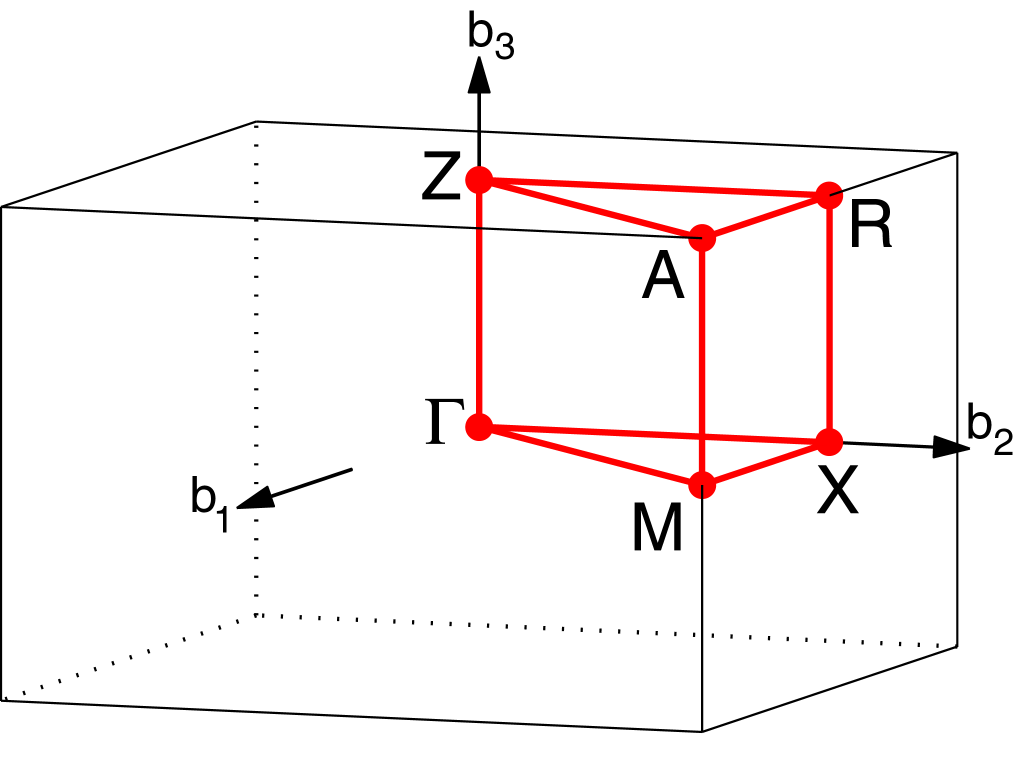
\includegraphics[width=0.5\textwidth]{figures/brillouin_zone}
    \caption{Brillouin zone of a tetragonal system, the red path passes through the high-symmetry points of the zone. $\vec{b}_1, \vec{b}_2, \vec{b}_3$ are the reciprocal base vectors of a tetragonal unit cell. The path used in the calculation of the band structure was $\Gamma$-X-M-$\Gamma$-Z-R-A-Z; X-R; M-A.}
    \label{fig:symmetry_points}
\end{figure}


As discussed in \cref{sec:dft+u}, DFT often fails to give appropriate results in band-gap calculation. To correct the problem, the previous calculations were repeated in the DFT+U approach. We followed the Duradev approach, setting the value of U to \SI{3.9}{eV} \cite{reticcioli2022}. The correction was applied to the d-orbitals of titanium, leaving the other unaltered. The band structure was computed along the same path described above.

To localize a polaron in the material, a unit cell is not enough. Since the unit cell is repeated in the crystal, the polaron could interfere with itself at the cell boundaries, resulting in self-interaction errors. To solve this problem, a supercell is used. A supercell is simply a cell made by the repetition of the unit cell. This is the main reason why only small polarons can be simulated in DFT: for large polarons, the supercell size would be too big to be simulated.

A $3\times3\times3$ supercell was created with the VESTA software \cite{zotero-174}, repeating the relaxed unit cell three times in each direction. A sketch of the supercell is reported in \cref{fig:supercell}. The same calculation described above were performed on the supercell. The output was analyzed and the number of electrons noted. This information was useful to trap an extra electron in the supercell.

\subsection{Electron localization}
The formation of the polaron is only slightly energetically favored compared to a delocalized solution, so the electron is difficult to localize. Simply adding an electron to the system does not result in a localized state, but the electron enters the conduction band and is delocalized in the crystal. This situation was also analyzed and compared with the polaronic solution. To achieve this, an extra electron was added to the supercell and a non-spin-polarized DFT+U calculation was performed. The extra electron was added manually, setting the NELECT flag in the INCAR file to the number of the electrons found in the previous step plus one.

To find a localized solution, a more gradual approach was necessary. To add an electron to the system, the central titanium atom was substituted with vanadium. Vanadium is the element following titanium in the periodic table, so it has one more electron and a stronger nuclear attraction. The substitution was done modifying the POSCAR and POTCAR files. For vanadium, a PAW pseudopotential with 13 electrons was used. Moreover, the six oxygen atoms around the central vanadium atom were moved outwards by \SI{0.04}{\angstrom}. A DFT+U calculation was run allowing lattice relaxations (\cref{app:localization}). $U-J$ was set to \SI{3.9}{eV} for titanium d-orbitals and to \SI{9}{eV} for vanadium d-orbitals. Together, the stronger nuclear attraction, the diplacement of the oxygen atoms, and the high $U-J$ value, favoured the electron localization on the central vanadium atom. The extra electron in the system introduced a spin magnetic moment, so the calculation was spin-polarized. The magnetic moment was initially set to zero for every atom except for the vanadium one, which was set to $+\mu_B$, where $\mu_B$ is the Bohr magneton.

To check if the electron was localized, the magnetic moment of the atoms was read from the OUTCAR file. For a localized state, we expected the central vanadium atom to be the only one with a magnetic moment (of 0.7-0.9 $\mu_B$). The localized solution was then used to initialize a new calculation. The goal was to gradually substitute the vanadium atom with a high $U-J$ value with a titanium atom with a normal $U-J$ value. This was done in two steps.

Firstly, vanadium was removed and titanium was placed back, and a second DFT+U calculation with lattice relaxation was run. To keep the electron in the system, the number of electrons was manually set to the same number of the calculation with vanadium. The $U-J$ value applied to the central atom was left unchanged. The same POSCAR - with the oxygen atoms shifted by \SI{0.04}{\angstrom} - was used. The calculation was initialized with the charge density and wavefunctions obtained from the system with vanadium, with the electron already localized. The calculation was spin-polarized, and the initial magnetic moment was read from the charge density file. The localization of the electron was checked looking at the magnetic moment as explained above. Moreover, the eigenvalues and DOS were also inspected to see if a new state was present in the middle of the band gap.

Secondly, the calculation of the polaron was done continuing the last calculation with a normal $U-J$ value for the central titanium atom. The calculation was initializes with the atomic positions, charge density and wavefunctions of the previous calculation. As the previous one, it was spin-polarized and the atomic positions were relaxed. The magnetic moments, DOS and eigenvalues were inspected again to check that the polaron was still present.

Some last simulations were run to compute the polaron properties. An electronic calculation without relaxation was done starting from the previous result to compute a more precise DOS. The band structure of the polaronic solution was also computed with a non-self-consistent calculation on the usual path of k-points. Finally, the isosurfaces of the charge density of the polaron was computed. To do so, the charge was decomposed over the different bands, and the polaronic band was selected restricting the calculation to an appropriate energy interval. The final result was rendered with VESTA, and the electron localization observed.